\documentclass[11pt]{report}
\usepackage[utf8]{inputenc}
\usepackage[margin=2.0cm]{geometry}
\usepackage{fancyhdr}
\usepackage{xcolor}
\usepackage{minted}
\usepackage{graphicx}

\title{Digital Engineering\\Lab 1}
\author{Y3890959\\Y3878784}
\date{24th January 2023}

\pagestyle{fancy}
\fancyhead{}
\setlength{\headheight}{14pt}
\fancyhead[L]{Lab 1}
\fancyhead[R]{Y3890959, Y3878784}
\fancyfoot{}
\fancyfoot[L]{Digital Engineering}
\fancyfoot[R]{\thepage}

\makeatletter
\let\ps@plain\ps@fancy 
\makeatother

\setminted {
    fontsize=\footnotesize,
    frame=single,
}

\begin{document}

\maketitle

\chapter*{Task A: Debouncer implementation and simulation by parameterization}

\section*{VHDL Code}

\subsection*{Top-Level Entity}
\inputminted{vhdl}{../../Lab1/Lab1.srcs/sources_1/imports/new/fibonacci_8bit_sequence.vhd}

\subsection*{Efficient (Updated) Debouncer Entity}
\inputminted{vhdl}{../../Lab1/Lab1.srcs/sources_1/new/efficient_debouncer.vhd}

\subsection*{Counter Entity}
\inputminted{vhdl}{../../Lab1/Lab1.srcs/sources_1/new/parameterizable_counter.vhd}

\subsection*{ROM Entity}
\inputminted{vhdl}{../../Lab1/Lab1.srcs/sources_1/imports/new/fibonacci_8bit_async_read_rom.vhd}



\section*{Testbenches and Simulation}

\subsection*{Testbech VHDL Code}
\inputminted{vhdl}{../../Lab1/Lab1.srcs/sim_1/imports/new/fibonacci_8bit_sequence_tb.vhd}



\subsection*{Testbench Waveforms}

\subsubsection*{Entire Sequence}
\begin{figure}[H]
    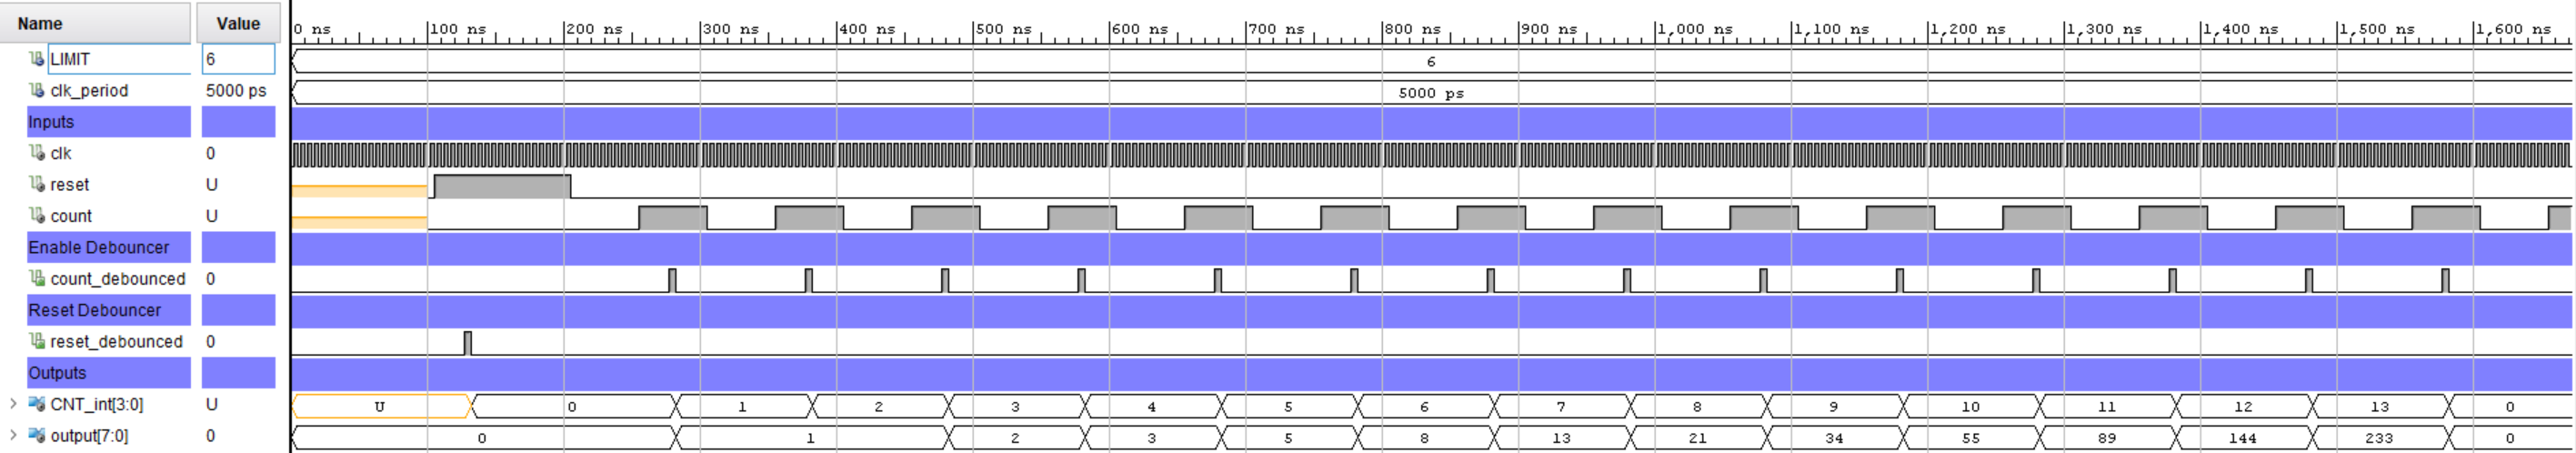
\includegraphics[width=\columnwidth]{Reports/Lab1/Waveforms/01_entire-sequence.png}
\end{figure}
The above waveform screenshot shows the entire sequence from time 0 to output 1 after a roll-over. This waveform is intended to verify that the overall output is correct.

\subsubsection*{Test 1, Waveform 1 - Initial reset and counting}
\begin{figure}[H]
    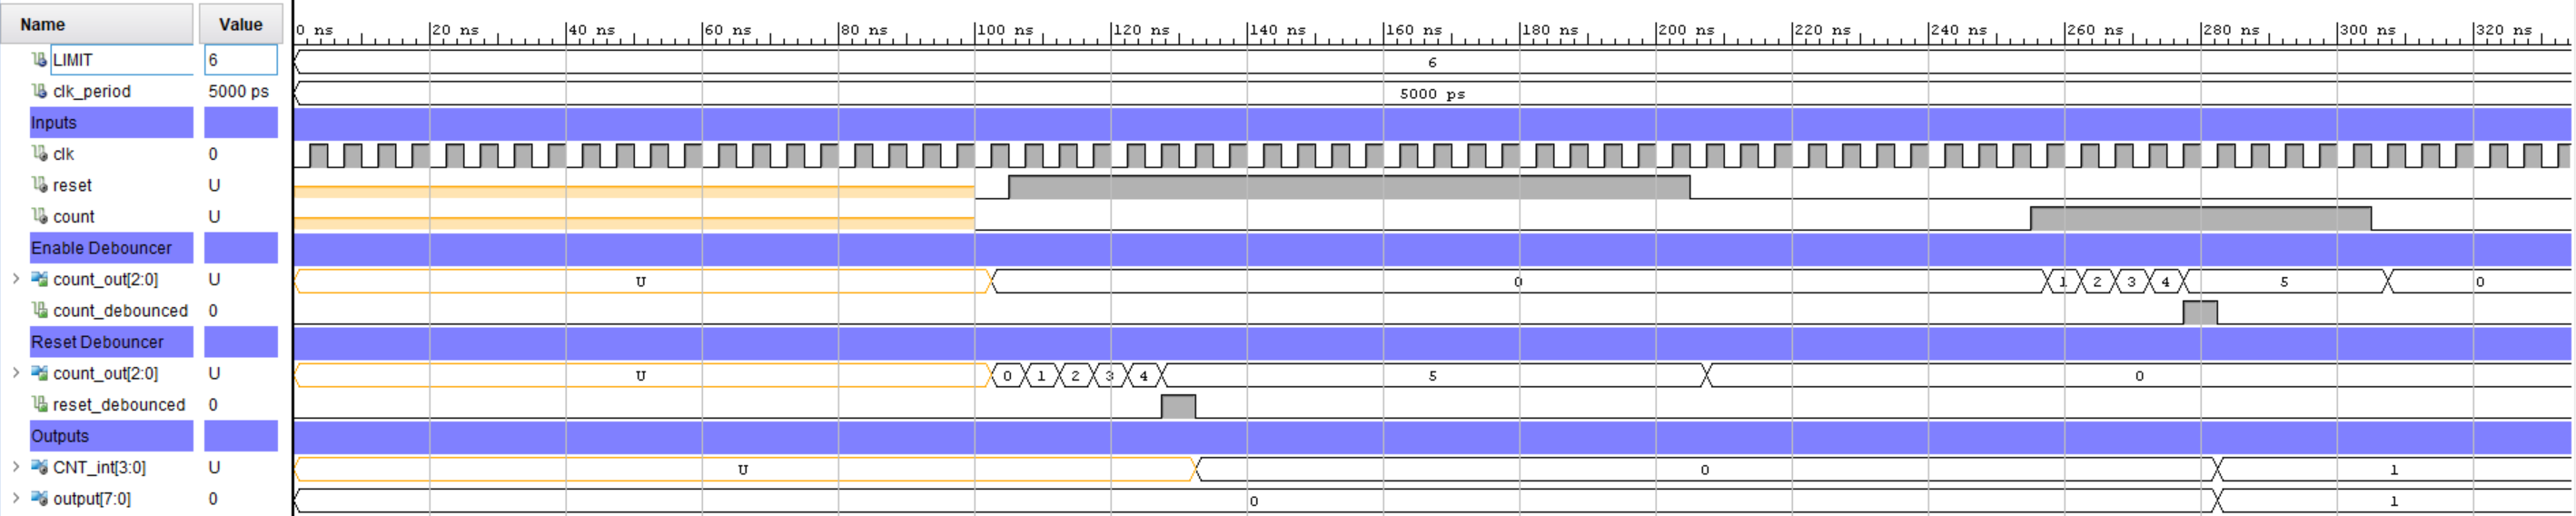
\includegraphics[width=\columnwidth]{Reports/Lab1/Waveforms/02_initial-reset-and-counting.png}
\end{figure}
The above waveform shows the initial global reset, verifying a successful activation of both the "reset" and "count" debouncers and a successful reset and increment of the overall circuit. 

\subsubsection*{Test 1, Waveform 2 - Counting up}
\begin{figure}[H]
    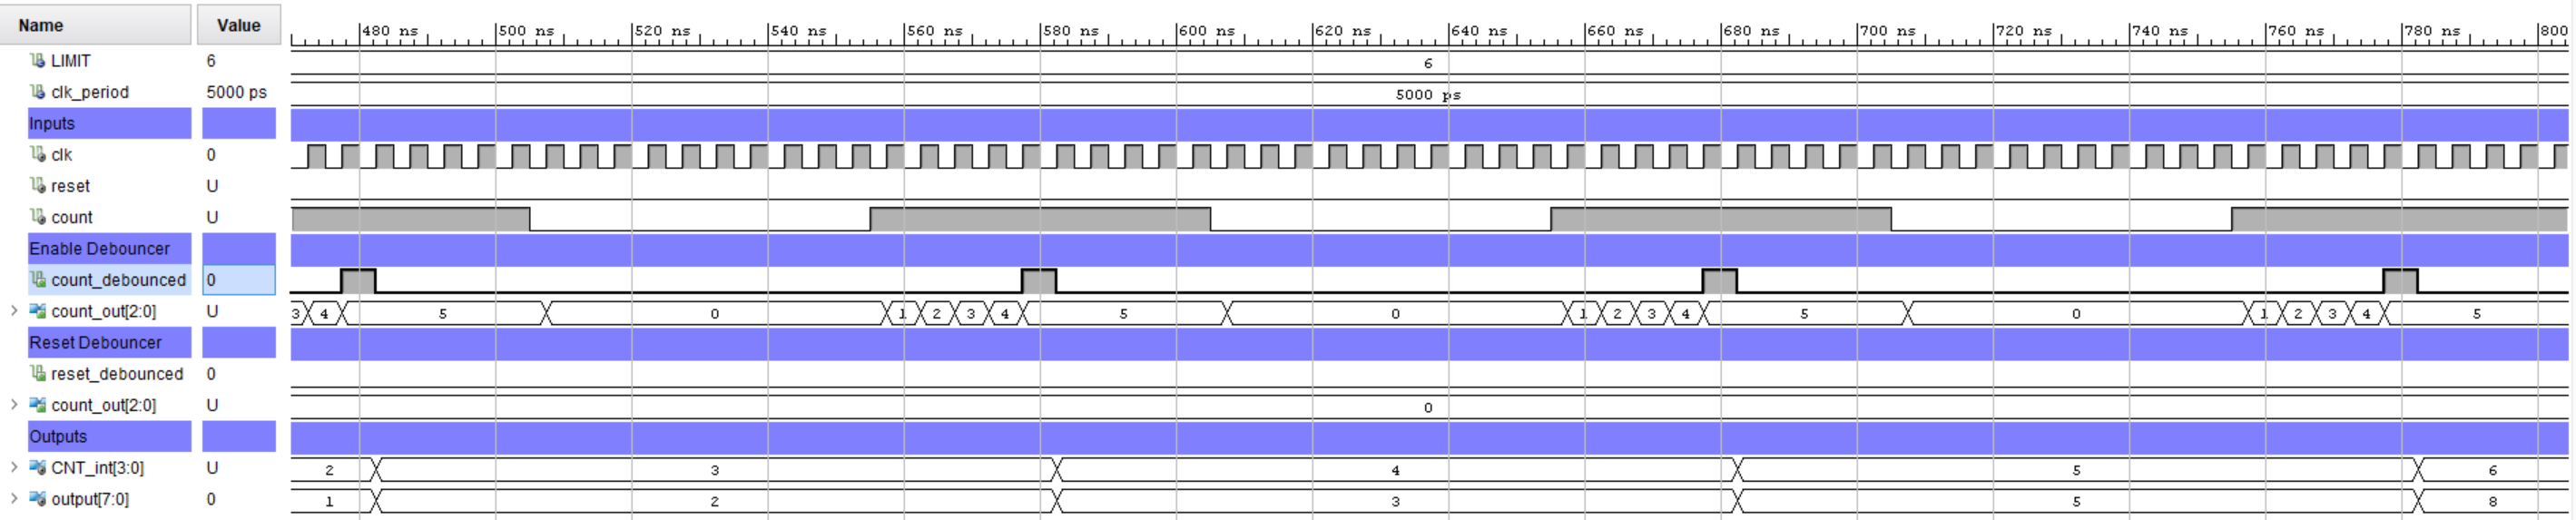
\includegraphics[width=\columnwidth]{Reports/Lab1/Waveforms/03_counting-up.png}
\end{figure}
This waveform (a continuation of Test 1, Waveform 1) verifies that the debouncer is activating and the counter is incrementing as designed, the Fibonacci sequence is shown (1,2,3,5,8).

\subsubsection*{Test 1, Waveform 3 - Roll-over and count up}
\begin{figure}[H]
    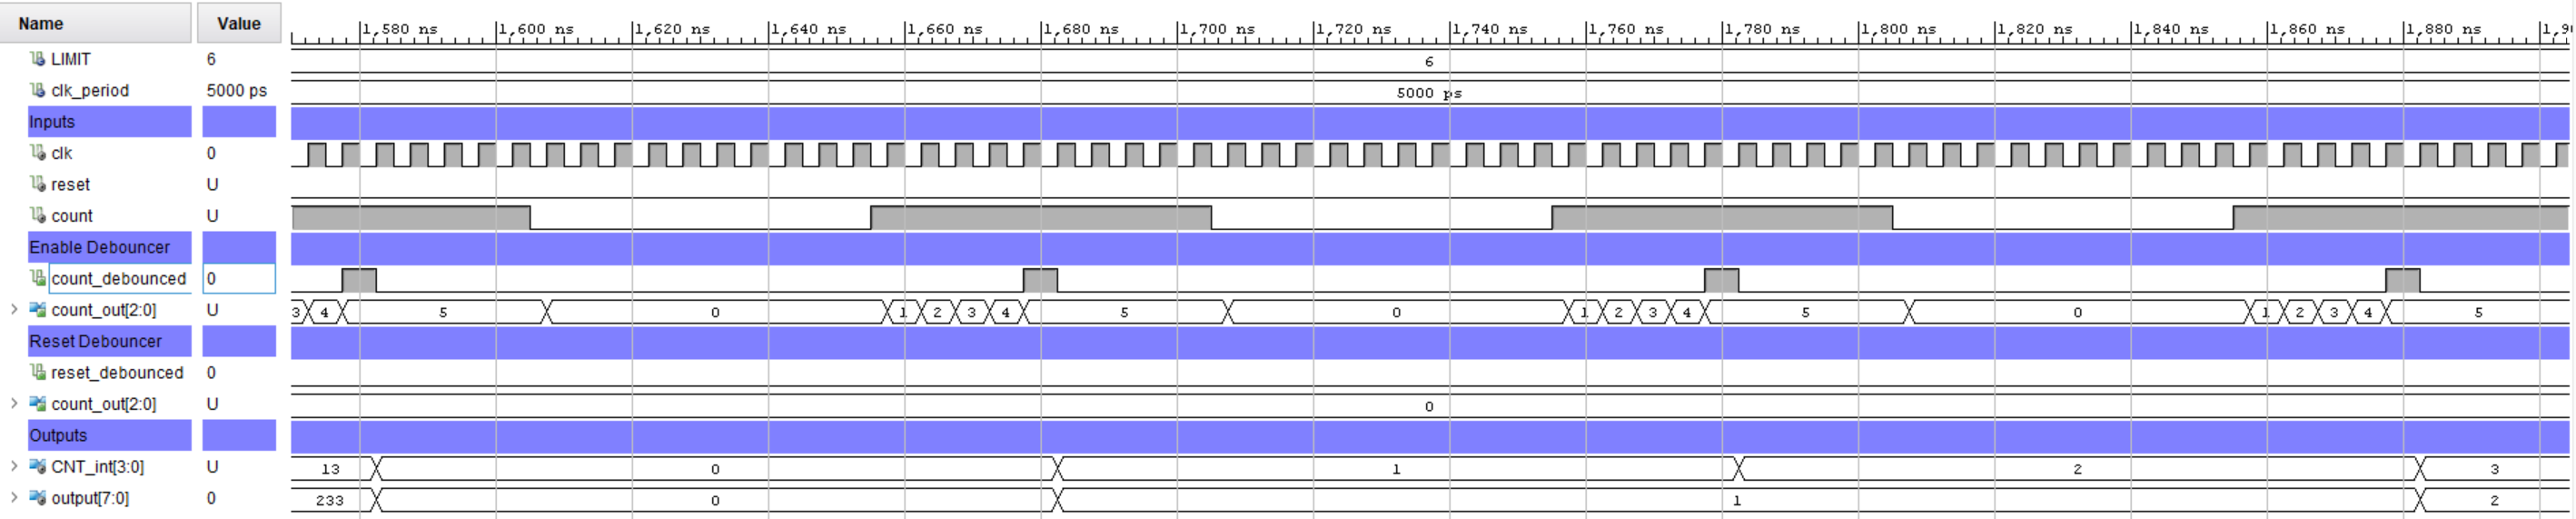
\includegraphics[width=\columnwidth]{Reports/Lab1/Waveforms/04_roll-over-and-count.png}
\end{figure}
This waveform verifies that the maximum Fibonacci sequence value is reached, and the sequence rolls over to 0 without a reset signal being generated by the user and can resume counting up.

\subsubsection*{Test 2 - Quick reset pulse}
\begin{figure}[H]
    \includegraphics[width=\columnwidth]{Reports/Lab1/Waveforms/}
\end{figure}
This waveform verifies that the maximum Fibonacci sequence value is reached, and the sequence rolls over to 0 without a reset signal being generated by the user and can resume counting up.



\section*{Circuit Analysis and Synthesis}

\subsection*{RTL Componenet Statistics}

\subsection*{RTL Hierarchical Component Statistics}

\subsection*{Schematics}

\subsubsection*{RTL Top Level (ROM Expanded)}

\subsubsection*{RTL Debouncer}

\subsubsection*{Synthesis Top Level (ROM Expanded)}

\end{document}
